\section{Experiment}
	\begin{figure}[htbp]
	\centering
	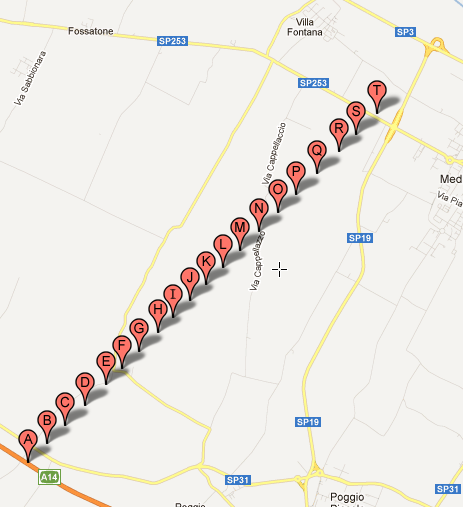
\includegraphics[width=3.4in]{imgs/punti_mappa.png}
	\caption{Fake positions used for the experiment}
	\label{fig:positions_experiment}
	\end{figure}

To test our testbed applications, we implemented Fast Broadcast algorithm (both for Android application and Desktop application). Simulation used a set of fake position distributed on a straight line, each at a random distance between $275$ and $325$ meters from the following. In figure \ref{fig:positions_experiment} a graphical representation can be seen. They covers approximately $8$ kilometers.

\subsubsection{Android application}
To test our Android application we used three Android devices. We executed Fast Broadcast algorithm whit the following parameters:

\begin{itemize}
	\item \ttt{SLOT SIZE 		= 100 ms} 
	\item \ttt{CW MIN 			= 5} 
	\item \ttt{CW MAX 			= 10}
	\item \ttt{ACTUAL RANGE 	= 900 m}
	\item \ttt{DEFAULT RANGE	= 300 m}
\end{itemize}

We first tried an execution wothout range estimation, then with range estimation phase. In the second case, the average amount of time waitd on the contention window by each device resulted to be smaller, and so the contention window size. However, due to the overhead introduced by Hello message exchanging and processing, a solution with static range performs a much faster message propagation.
In both cases, the overhead introduced by TCP traffic doesn't let the algorithm beahave properly, resulting in some cases in simultaneous message forwarding by different devices.
